\documentclass[12pt]{article}
\usepackage[utf8]{inputenc}
\usepackage{glossaries}
\usepackage{amsmath}
\usepackage[german]{babel}
\usepackage{hyphenat}
\usepackage{graphicx}
\usepackage{setspace}

\def\changemargin#1#2{\list{}{\rightmargin#2\leftmargin#1}\item[]}
\let\endchangemargin=\endlist 

\graphicspath{ {/images} }

\begin{document}
\onehalfspacing

\titlepage{
    \vspace{1cm}

    \begin{center}
        \large{
            \begin{center}
                Gymnasium Nepomucenum Coesfeld \\
            \end{center}

            Besondere Lernleistung im Abitur 2022
        }
    \end{center}
    \vspace{0,1cm}
    \begin{center}
        
\includegraphics[width = 5cm, height = 2.5cm]{Nepo_Logo.png}
    \end{center}
    \vspace{0,1cm}
    \begin{center}
        \Large{ \textbf{DMergency - App zur Alarmierung und Verwaltung von Sanitätsdiensten\\}}
    \end{center}
    \vspace{0,1cm}
    \begin{center}
        \large Entwicklung einer App zur effizienten und benutzerfreundlichen Alarmierung, sowie Verwaltung von Sanitätsdiensten
    \end{center}

    \begin{center}
        \vspace{0,5cm}
        \large vorgelegt von\\
        \vspace{1cm}
        \LARGE{\textbf{Mattis Rinke}}
    \end{center}

    \begin{center}
        \large{
            \vspace{2cm}
            Fachbereich Informatik\\
            \vspace{1cm}
            Herr Brumma\\
            Herr Willenbring
        }
    \end{center}
    \vspace*{\fill}

}
\newpage
\thispagestyle{empty}
\tableofcontents
\thispagestyle{empty}

\newpage
\section{Einleitung}
\setcounter{page}{3}
    In der heutigen Welt wird der Drang nach Digitalisierung immer größer, wie auch bei Sanitätsdiensten.
    Die habe ich selbst durch meine Tätigkeit im Schulsanitätsdienst erfahren. Hier wurde bisher meist mit
    Funkgeräten oder auch mit Schuldurchsagen alarmiert, was den Schulunterricht drastisch gestört hat.
    Außerdem ist die Alarmierung selbst sehr ineffizient, da zunächst eine Person im Sekretariat oder ähnlichem 
    informiert werden muss, die anschließend dann die Sanitäter/-innen alarmiert.\\ 
    Dieses Problem wollte ich angehen, sodass ich mich zusammen mit einem Freund zusammen daran gesetzt habe dieses
    Problem zu lösen. Durch meine Vorkenntnisse im Fach Informatik bin ich dann schnell auf die Idee gekommen
    die Alarmierung per App zu gestalten. 
    Ich habe mich dann, als ich bereits angefangen hatte die App zu programmieren von der Möglichkeit erfahren
    eine besondere Lernleistung in das Abitur einfließen zu lassen, dazu entschieden dies zu tun.\\
    In dieser Ausarbeitung gehe ich darauf ein, wie die App entstanden ist, warum ich mich für das Framework Flutter
    entschieden habe, welche Funktionen die App hat und wie diese umgesetzt wurden.\\
    Als erstes werde ich skizzieren, was die App warum können soll und beschreibe im Anschluss, wie ich mich von der nativen 
    Entwicklung zur Nutzung des Cross-Platform-Frameworks Flutter entschieden habe.
    Danach erkläre ich detaillierter die einzelnen Funktionen der App, woraufhin die Kommunikation mit dem Server und die
    Speicherung der Daten näher erörtert wird. Zuletzt führe ich noch Ergebnisse der ersten Schultests auf und 
    ziehe dann ein Fazit, in dem ich erkläre, was in der Ausarbeitung bereits geschafft wurde und wie ich mit der App
    weiterhin verfahre.

\section{Das Projekt}
\subsection{Zielsetzung}
    Die App soll das Alarmieren und Verwalten von Sanitätsdiensten vereinfachen. Um dies
    zu verwirklichen ist es erforderlich mehrere Funktionen zu implementieren. Zum 
    einen ist eine Funktion zum Alarmieren unerlässlich, welche zur Vergewisserung für
    die alarmierende Person auch ein Feedback anzeigen sollte, zum anderen sollte es 
    dann auch eine Funktion zum Empfangen des Alarms geben. Diese beiden Funktionen 
    sollten so implementiert werden, dass eine alarmierende Person so wenig Aufwand wie 
    möglich in der Durchführung der Alarmierung hat, die Sanitäter/-innen jedoch trotzdem 
    so viele Informationen wie möglich bekommen. Damit eine Verständigung seitens der 
    Sanitäter/-innen darüber erzielt werden kann, wer sich für das Einsatzmaterial 
    verantwortlich zeigt, ist es erforderlich, dass dies ebenfalls mit in die Funktionen 
    aufgenommen wird.
    Darüber hinaus ist die Programmierung eines Dienstplan-Systems vorgesehen, das nur
    diensthabende Sanitäter/-innen alarmiert.
    Selbstverständlich gibt es im (Schul-)Alltag auch Situationen, in denen Sanitäter/-innen
    kurzfristig (z.B. im Falle von Krankheiten) oder auch absehbar längerfristig (z.B.
    durch angekündigte Arbeiten, Ausflüge oder Praktika) ihren Dienst nicht durchführen 
    können, so dass es eine Funktion geben muss, mit der sich diese austragen können und
    andere ihren Dienst übernehmen.
    Im Notfall ist eine schnelle Rettungskette von großer Bedeutung. Um diese Hilfskette
    \cite{Rettungskette} einzuhalten, sollen in der App wichtige Notfallnummern hinterlegt
    werden, welche dann durch einen schnellen Klick wählbar sind.
    
    Ein weiterer wichtiger Bestandteil zur Verwaltung des Sanitätsdienstes 
    ist die Kommunikation zwischen der Leitung und den Mitgliedern des Sanitätsdienstes.
    Um diese Kommunikation sicherzustellen soll eine News-Funktion programmiert werden, 
    in welcher die Mitglieder Neuigkeiten von der Leitung einsehen können.
    Hierzu ist es unabdingbar eine Funktion umzusetzen, die es der Leitung ermöglicht,
    "News schreiben" zu können.

\subsection{Abgrenzung zur Server Ausarbeitung}
    In dieser Ausarbeitung wird die Funktionsweise der App \glqq DMergency" \grqq{} 
    beschrieben und wie sie in Zusammenarbeit mit dem Server arbeitet. Es wird nicht 
    darauf eingegangen, wie der Server arbeitet und welche Funktionen es in der 
    Web-Anwendung gibt. Zum Teil werden Daten vom Server verarbeitet oder auf diesem 
    gespeichert. In diesen Fällen wird dies erwähnt jedoch nicht weiter auf die
    Verarbeitung eingegangen.
\section{Wahl der Entwicklungsweise}
    Es gibt in der Programmierung etliche Möglichkeiten der Programmierung. Auch in der 
    Entwicklung für mobile Endgeräte. Mit dem Projektstart wählte ich den mir zunächst am 
    sinnvollsten erscheinenden Weg der nativen Entwicklung.
    Die native Entwicklung. Dadurch, dass die App für unterschiedliche Betriebssysteme 
    erhältlich sein soll, muss die native Entwicklung sowohl für das Betriebssystem iOS 
    \cite{iOS} von Apple durchgeführt werden, als auch für das Betriebssystem Android 
    \cite{Android}, von Google.
    Es gibt aber auch die Möglichkeit der Cross-Platform-Programmierung, bei 
    der für beide Betriebssysteme gleichzeitig programmiert wird. 
    Wie schon erwähnt, entschied ich mich zunächst für die native Programmierung, jedoch 
    bewegte ich mich im Entwicklungsprozess von der nativen Entwicklung zur Cross-Platform-
    Programmierung mit dem Framework Xamarin-Forms, um schließlich das Framework Flutter zu 
    verwenden. Worin die Vor- und Nachteile liegen und warum ich mich letztendlich für die 
    Cross-Platform-Programmierung mit Flutter entschied wird in den nächsten drei 
    Unterkapiteln erläutert.

\subsection{Version 1 - Native Entwicklung}
    Der Einstieg in die native Entwicklung erfolgte mit Android, da hier für mich eine 
    garantierte Kompatibilität mit dem Betriebssystem vorlag. Diese stellte sich als mühelos
    heraus, da in der Programmiersprache Java geschrieben wird, die mir aus dem Informatik-
    Unterricht bereits bekannt war.
    Nach kurzer Zeit lag eine vorläufig fertig programmierte App vor, die einen zuverlässigen 
    Empfang und das Auslösen eines Alarms ermöglichte. Da dieser App jedoch auch zuerst nur 
    für den Schulsanitätsdienst meiner eigenen Schule gedacht war gab es hier kein Registrier-
    und Login-Verfahren genauso wenig wie die Notfallnummern, die News und die Einstellungen.
    Diese App war also nur auf den Sanitätsdienst meiner eigenen Schule zugeschnitten.

    Da es jedoch auch iOS-Geräte in diesem Sanitätsdienst gibt, musste ich schnell merken, 
    dass ich auch hier eine App programmieren muss. Also habe ich mich informiert und habe 
    wie ich für iOS entwickle und die App auch für iOS-Geräte veröffentlichen kann.
    Die Programmierung für iOS findet nativ in den Programmiersprachen Swift und Objective-C
    statt, was mich vor ein weiteres Problem gestellt hat. Ich bin weder mit der Programmiersprache
    Swift noch mit der Programmiersprache Objective-C vertraut, was bedeuten würde, dass ich mir
    diese von null auf beibringen müsste. Dies wäre zwar sehr unangenehm, jedoch möglich gewesen.
    Ich habe jedoch erst ein Mal weiter recherchiert und bin auf die nächste Barriere gestoßen:
    Um die App veröffentlichen zu können muss ich einen Apple-Developer-Account haben um die App
    im Appstore veröffentlichen zu können. Da diese 99€ im Jahr kostet bin ich zu dem Entschluss 
    gekommen, dass es für mich nicht möglich ist die App nur für den Sanitätsdienst meiner eigenen Schule
    zu entwickeln. Um dieses Problem zu umgehen habe ich mich dazu entschieden die App nicht 
    nur für meinen eigenen Sanitätsdienst zu entwickeln, sondern diese auch an weitere Sanitätsdienste
    zu verkaufen. Um dies zu bewerkstelligen musste ich jetzt also zum einen die App sowohl für
    Android, als auch für iOS zu entwickeln, da der Marktanteil von Apple bei 30\% und der von Google bei
    70\% liegen\cite[vgl.]{Marktanteil}. Bei der nativen Entwicklung müsste ich jetzt also 
    den Code für das \glqq gleiche\grqq{} Produkt zweimal schreiben, da ich die App einmal in
    Objective-C/Swift und einmal in Java/Kotlin schreiben müsste.
    Dies ist als Einzelperson nicht machbar, weshalb ich mich neu orientierte. 
    Recherchearbeiten führten mich dann zu der Methode des Cross-Platform-
    Programmings, welche in den nächsten zwei Unterkapiteln erläutert werden.

\subsection{Version 2 - Xamarin Forms}

    Xamarin Forms ist ein Framework der \textbf{.NET-Plattform} von Microsoft. Dieses 
    Framework ist ein Cross-Platform-Framework, das heißt, dass der Code einmalig für 
    die beiden Betriebssysteme (Android \& iOS) geschrieben wird und die App dann für 
    beide erhältlich ist. Xamarin Forms hat eine Unterteilung zwischen dem funktionalen 
    Code, welcher in C\# geschrieben ist, und zwischen der der Markup Language XAML, 
    welche das GUI darstellt\cite[vgl.]{Xamarin}. Jedoch sind bei der Nutzung von Cross-
    Platform-Frameworks auch Einbußungen zu machen. In diesem Fall konnte ich mich zum 
    einen nicht mit der Markup Language XAML anfreunden, da hier das neu laden des GUIs 
    als sehr sperrig und aufwendig herausstellte, zum anderen stellte sich heraus, dass 
    Xamarin einige von mir benötigte Funktionen nicht voll oder gar nicht unterstützt. 
    Unter anderem gab es immer wieder Probleme beim Einbinden von Firebase-Messaging, ein
    Tool von Google, zum Versenden von Push-Notifications (Auf Firebase-Messaging wird im
    weiteren Verlauf der Ausarbeitung noch eingegangen).
    Durch diese für mich nicht lösbaren Probleme musste ich mich dann erneut auf die Suche
    nach einer anderen Lösung machen. Um diese Lösung geht es jetzt im nächsten Abschnitt.

\subsection{Version 3 - Flutter}

    Die dritte und bis jetzt finale Version ist in Flutter geschrieben und die am weitesten 
    entwickelte App-Version. Die Entscheidung für Flutter viel nach mehreren Empfehlungen, 
    z.B. durch einen Freund, welcher bereits durch ein Praktikum bei der Firma d.velop mit 
    diesem Erfahrung sammeln konnte, sowie nach eigener Recherche. Flutter nutzt eine 
    einfache Programmiersprache, die Java ähnelt, weshalb mir der Einstieg in die 
    Programmiersprache Dart\cite{Dart} nicht schwergefallen ist. Flutter ist wie Xamarin-Forms
    ein Cross-Platform Framework. Dieses ist in der Lage Apps für die beiden gängigen 
    Plattformen iOS und Android zu kompilieren\footnote{Kompilieren beschreibt das Umwandeln
    des geschriebenen Programmtextes in ein funktionsfähiges Programm}, sowie für das Web.
    Das Nutzer-Interface ist in Flutter durch so genannte Widgets, welche in einem Widget-
    Tree aufgenommen werden, dargestellt. Hierbei wird dann zwischen \glqq Stateless\grqq
    \cite{Stateless-Widget}- und \glqq Stateful\grqq\cite{Stateful-Widget}-Widgets unterschieden. 
    Der Unterschied liegt darin, dass in \glqq Stateless-Widgets\grqq{} zwar Variablen, etc. abgeändert 
    werden können, jedoch wird das Widget im GUI nicht neu gerendert. Es können aber in dem 
    Widget selbst andere Widgets, die selbst \glqq Stateful-Widgets\grqq{} sind, aktualisiert werden.
    Ein Stateful-Widget besteht aus zwei Klassen. Der Klasse, die um die Klasse 
    \glqq Stateful-Widget\grqq{} erweitert wird und der Klasse, die um die Klasse 
    \glqq State\grqq{}\cite{State} erweitert wird. In der Klasse mit dem Stateful Widget wird in der
    \glqq createState\grqq{}-Methode die Klasse mit dem State zurückgegeben. Der eigentliche Widget-Tree
    wird dann erst in der \glqq build-Methode\grqq{} der State-Klasse geschrieben und dann auch 
    zurückgegeben. Nach der Erstellung des Widget-Trees kann bei Bedarf durch die Methode 
    \glqq setState\grqq{} das UI aktualisiert werden. Außerdem gibt es asynchrone Methoden und 
    Futures\cite{Futures}. Diese sind dazu da das Programm weiterhin Code ausführen zu lassen,
    während das Programm gleichzeitig darauf wartet, dass die asynchrone Methode fertig wird. 
    Dies wird oft dazu genutzt Daten vom Netzwerk zu laden oder in eine Datenbank zu 
    schreiben. Die meist genutzten Datentypen sind: int, String, bool, List, Future und Map.
    Nach einiger Überlegung und Recherchen ist die Entscheidung letztendlich für flutter als 
    Framework gefallen, weil zum einen nur einmal Code für die beiden Plattformen iOS und 
    Android geschrieben werden muss und zum anderen das GUI einfacher programmierbar ist als 
    z.B. mit Xamarin Forms und Flutter sehr performant ist. In dieser Version sind die Funktionen
    der Alarmierung, des Alarm Empfangens, der Vertretung für den aktuellen Tag, das wählen von 
    Notfallnummern, die News und die Einstellungen implementiert.

\section{Entwicklung}
\subsection{Funktionen der App}
        In den folgenden Abschnitten werden die Funktionen der App dargestellt 
        und erklärt. Im Kontext der jeweiligen Funktion werden beispielhaft einzelne 
        Methodenimplementationen herausgenommen,erklärt  und erörtert.
        Außerdem werden Design-Entscheidungen skizziert um die Nutzer-Erfahrung zu 
        visualisieren.   
        
\subsubsection{Rollen und Registrierung}
        Wie bereits in der Zielsetzung dargestellt, soll es ein Berechtigungssystem 
        für die App geben. Unterteilt wird dieses in die Rollen \glqq Sanitäter/-in\grqq{} 
        und \glqq Alarmierende/-n\grqq{}. Alarmierende sollen nur in der Lage sein einen Alarm 
        auszulösen und die Alarmierenden-News, sowie die Notfallnummern einzusehen.
        Anders als die Alarmierenden sollen Sanitäter/-innen auch in der Lage sein 
        einen Alarm zu empfangen und andere Sanitäter/-innen zu vertreten oder sich 
        aus dem Dienstplan auszutragen. Um dies umzusetzen muss bereits bei der 
        Registrierung darauf geachtet werden, wer welche Rolle zugewiesen bekommt.
        Im Folgenden erkläre ich jetzt, zunächst beispielhaft, wie die Registrierung 
        für eine/-n Sanitäter/-in abläuft und erläutere im Anschluss, welche Unterschiede es 
        bei der Registrierung für Alarmierende gibt.
        \newline\\
        Zunächst muss der/die Nutzer/-in den ihr/ihm zugehörigen Sanitätsdienst 
        auswählen. Um diesen auszuwählen muss der / die Nutzer/-in auf 
        den gewünschten Sanitätsdienst klicken. Wenn dieser nicht direkt erscheint, 
        ist es außerdem möglich diesen mit der im View (Mit dem Wort View beschreibe ich die unterschiedlichen
        Benutzeroberflächen, welche ich implementiert habe) oben angelegten Suchleiste herauszusuchen.  
        Im Anschluss muss der/die Nutzer/-in auf den \glqq Weiter\grqq{}-Button klicken um sich
        darauf folgend anzumelden oder zu registrieren. 
        Zusätzlich verdeutlicht der Button durch unterschiedliche Farbanzeige, ob ein Anklicken erfolgen kann oder nicht.
        Erscheint der Button grau, ist ein Anklicken nicht möglich und macht deutlich, dass bisher kein Sanitätsdienst 
        ausgewählt wurde. Erscheint der Button in der Farbe grün, besteht die Möglichkeit den Button anzuklicken, da bereits
        ein Sanitätsdienst ausgewählt wurde.
        \\In Abbildung 1 ist der View zu sehen, 
        in welchem der Sanitätsdienst ausgewählt wird.
        
        %\begin{figure}[H]
        %    \begin{center}
        %       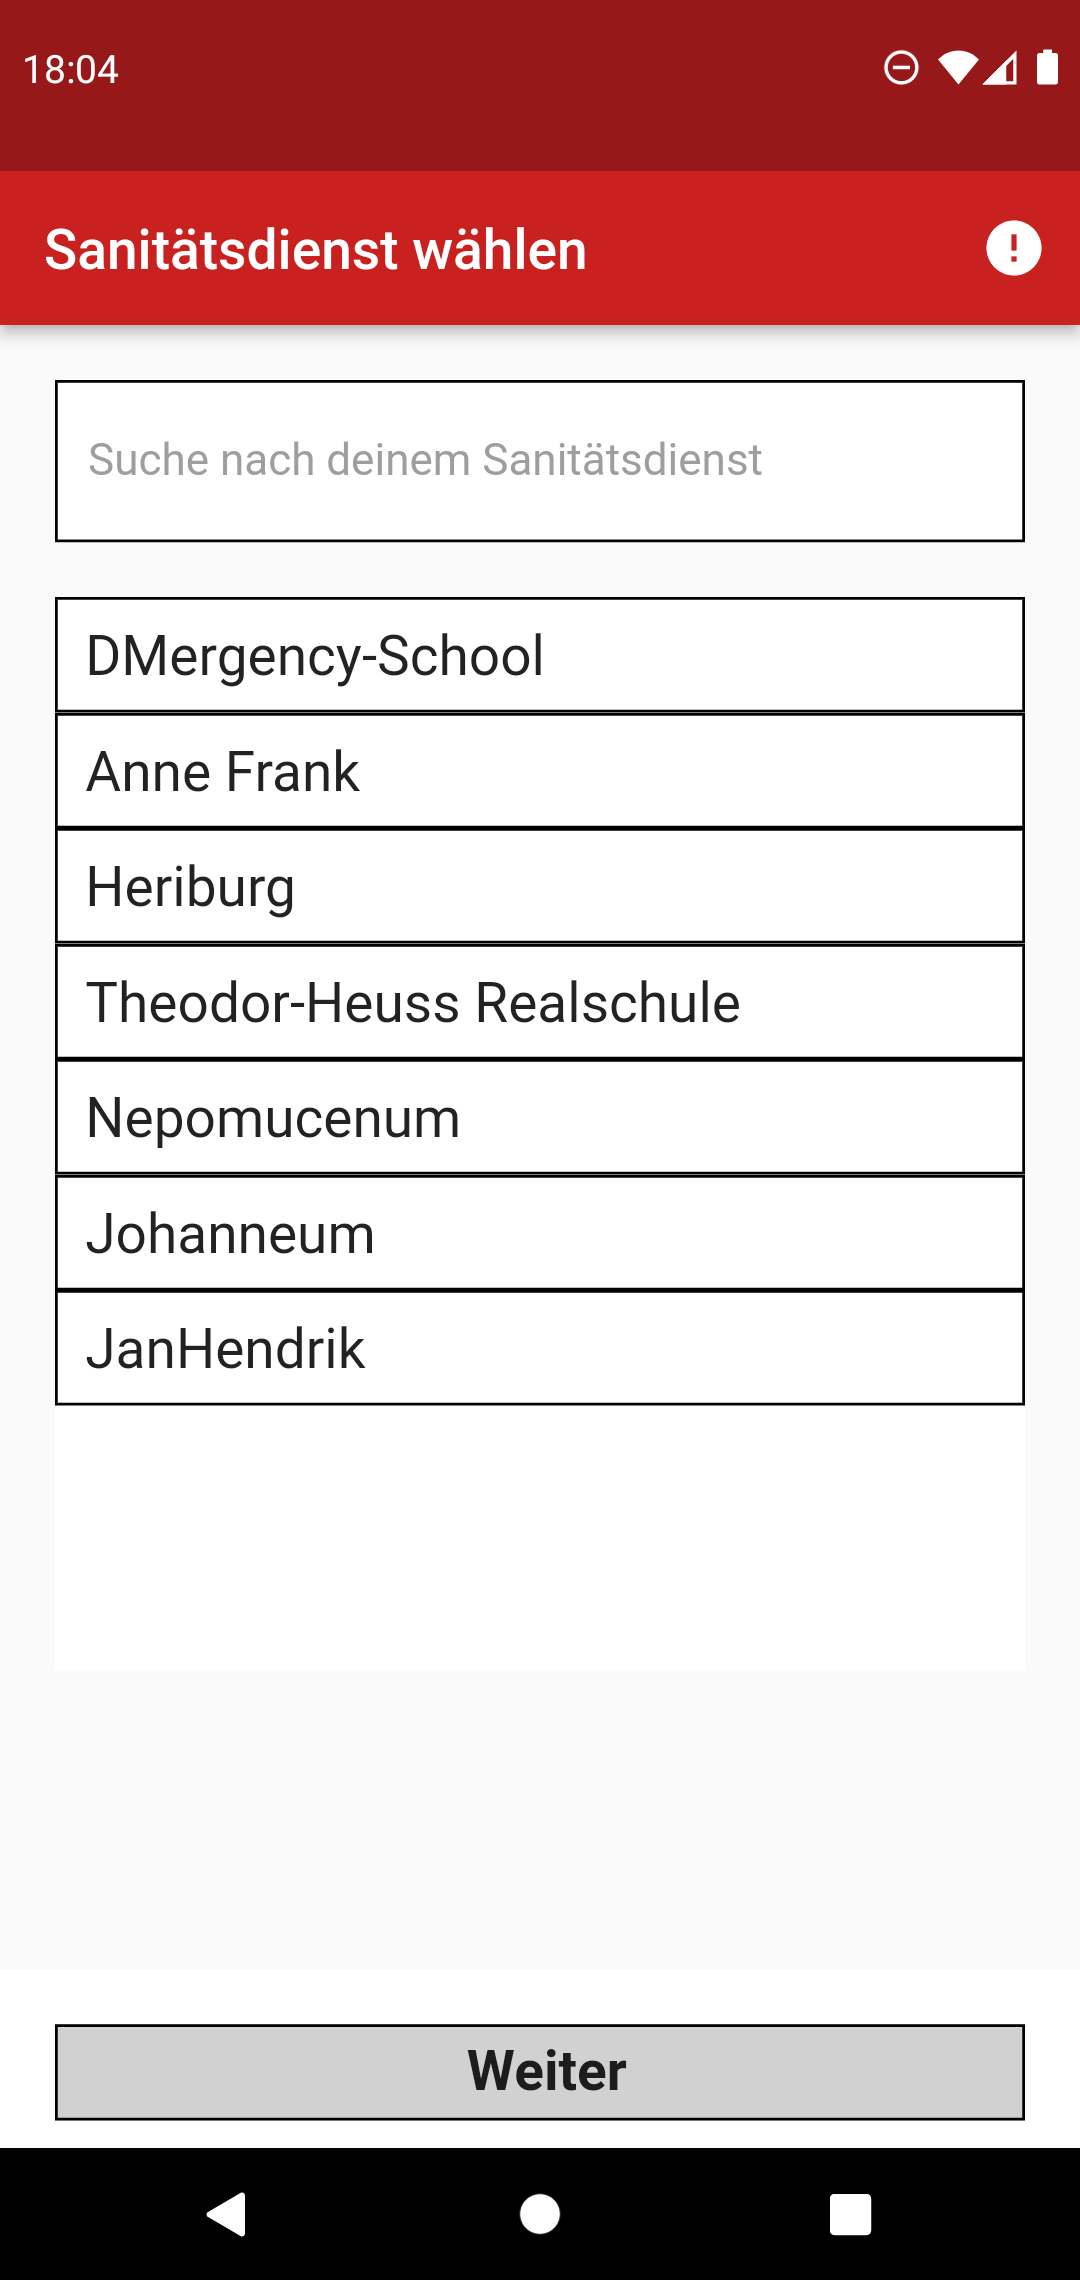
\includegraphics[width = 5cm]{images/SanitaetsdienstWahl.png}
        %    \end{center}
        %    \caption[Screenshot der Sanitätsdienst-Auswahl]{Beispielhafte Sanitätsdienst-
        %Auswahl}
        %\end{figure}
        
        \noindent Um vorher beschriebenes umzusetzen, muss beim Start der App zunächst überprüft werden, 
        ob bereits ein Nutzer eingeloggt ist oder nicht.
        \newline
        1. Es muss überprüft werden, ob schon ein Nutzer eingeloggt ist. In diesem 
        Fall soll keine Sanitätsdienstauswahl angezeigt werden, sondern
        die normale Nutzeroberfläche, für die entsprechende Rolle.
        \newline
        2. Ist bisher kein Nutzer eingeloggt, muss die Sanitätsdienstauswahl 
        angezeigt werden und die wählbaren Sanitätsdienste vom Server geladen 
        werden.
        \newline\\
        Nachdem der/die Sanitäter/-in dann seinen/ihren Sanitätsdienst ausgewählt hat,
        soll nun ein Login-View angezeigt werden, bei welchem der/die Nutzer/-in sich entscheiden 
        kann ob er/sie:
        \newline
        1. sich einloggen möchte.
        \newline
        2. sich neu registrieren möchte.
        \newline
        3. sein/ihr Passwort vergessen hat und dieses zurücksetzen möchte.
        \newline\\
        In der Nutzeroberfläche ist dies so umgesetzt, dass je ein Eingabefeld für
        die E-Mail-Adresse und das Passwort angegeben ist. Unter diesem sind dann je
        zwei Textfelder angelegt: \glqq Registrieren\grqq{} und \glqq Passwort vergessen\grqq{}, über
        welche dann auf die unterschiedlichen Views geleitet wird. Ganz unten in dem
        View erscheint dann erneut ein Button, welcher zum Anmelden genutzt werden 
        kann (Auch hier gibt es wieder die Unterscheidung wählbar/nicht wählbar).
        \\
        Im Code habe ich dies so umgesetzt, dass in einem View \glqq Validate\grqq{} ein 
        \glqq FutureBuilder\grqq{} zurückgegeben wird, der so lange einen LoadingIndicator angezeigt
        (Also einfach nur einen sich drehenden Kreis, der an einer Stelle eine Lücke hat)
        bis die \glqq future\grqq{} ausgeführt wurde. Die \glqq future\grqq{} ist eine Methode, welche 
        \texttt{async} (also asynchron) ist. In diesem Fall wird durch diese Methode die Rolle des/der Nutzer/-in 
        bestimmt. Hierfür werden zunächst die Login-Daten aus der Datenbank gelesen und 
        überprüft ob diese vorhanden sind. Danach wird kontrolliert, welche Nutzer/-innen Rolle in der 
        Datenbank steht und diese je nachdem passend für die API abgeändert (In der lokalen
        Datenbank ist 0 gespeichert, was für eine/-n Sanitäter/-in steht $\rightarrow$ 
        Abänderung zu 3, da ein/-e Sanitäter/-in bei der API eine 3 ist). Danach wird durch 
        eine Anfrage an den Server geprüft, ob der Nutzer noch existent ist, indem die 
        Sanitätsdienst-ID, die Nutzer-ID und die Rolle als \glqq query-Teil\grqq{} mitgegeben. Danach 
        wird abgeglichen, was die Antwort des Servers ist. Ist diese eine 0 wurde der Account 
        gelöscht und der/die Nutzer/-in wird ausgeloggt und auf die Sanitätsdienstauswahl 
        geleitet. Ist die Antwort eine 2, wird der/die Nutzer/-in auf den View der eigenen 
        Rolle weitergeleitet, kann jedoch keine Alarme versenden, da der Account 
        vorübergehend gesperrt ist. Bei diesen beiden Fällen wird jeweils ein AlertView 
        angezeigt, der darüber informiert, was \glqq falsch\grqq{} gelaufen ist (Zum Beispiel könnte
        hier dann angezeigt werden, dass der Account gesperrt ist).
        Dies ist implementiert worden, da die Administrator/-innen in der Lage sind Accounts zu löschen
        oder zu sperren, damit Nutzer/-innen, die die App ausnutzen gesperrt werden können.
        Im Falle einer 1 als Antwort ist alles normal und der/die Nutzer/-in wird auf den 
        passenden View für die jeweilige Rolle weitergeleitet. 

        \noindent Damit eine Anmeldung erfolgen kann, ist es notwendig einen bereits angelegten Account zu besitzen,
        den man auch in der App registrieren kann. Im Login-View die Eingabe der E-Mail-Adresse, 
        die mit dem Account verknüpft ist, sowie des zugehörigen Passwortes, um das Einloggen zu ermöglichen. 
        Die Account-Daten werden nach der Login-Bestätigung
        durch die App zum Server geschickt und überprüft, um dem/der Nutzer/-in
        im Anschluss eine Fehler-Meldung anzuzeigen oder sie/ihn auf die 
        Nutzeroberfläche weiterzuleiten.

        Um das Passwort zurücksetzen zu können, muss ein neuer \glqq View\grqq{} geöffnet werden, 
        in dem die persönliche E-Mail-Adresse eingegeben werden kann. Nachdem der/die Nutzer/-in
        diese bestätigt hat, erhält der/die Nutzer/-in eine E-Mail an die angegebene E-Mail-Adresse, die das
        Zurücksetzen des Passwortes ermöglicht.

        Das Registrier-Verfahren ist komplizierter. Nach dem Aufruf von \glqq Account erstellen\grqq{}
        Account erstellen ist es notwendig ein Passwort zur Registrierung anzugeben, dass
        durch die Leitung des Sanitätsdienstes festgelegt wurde. Dieses Passwort unterscheidet sich
        je nach Rolle, die zugeteilt werden soll. Das heißt: Nutzer/-in A soll die 
        Rolle Sanitäter/-in bekommen, so dass er/sie Passwort \glqq xyz\grqq angibt.
        Nutzer/-in B soll die Rolle Alarmierende/-r bekommen, also gibt die Person 
        Passwort \glqq abc\grqq an.
        \newline
        Nach der Verifizierung dieses Passworts erfolgt die weitere Registrierung der Rollen unterschiedlich: 
        \\\\
        1. Registrierung des/der Sanitäter/-in
        \newline Zunächst müssen Sanitäter/-innen ihren Vor- und Nachnamen zur 
        Identifizierung für die Sanitätsdienst-Leitung angeben. Außerdem muss eine 
        Stufe (bestehend aus drei beliebigen Zeichen) und ein Geschlecht angeben. 
        Diese Daten dienen der Sanitätsdienst-Leitung zur Identifizierung und Planung
        des Sanitätsdiensts. Dies Daten werden zum Beispiel für die Dienstplanung
        verwendet, da dieser möglichst divers sein sollte und nicht nur unerfahrene Sanitäter/-innen
        im Dienst sein sollen.\\ Danach muss der/die Nutzer/-in eine E-Mail-Adresse und
        ein Passwort angeben, um sich wieder anmelden zu können und den Nutzer im 
        System eindeutig zu identifizieren. Um sicher zu gehen, dass das gewünschte Passwort angegeben wurde,
        muss dieses zweimal eingegeben werden.
        Im Anschluss daran werden App-Berechtigungen abgefragt. Warum es diese
        gibt und weshalb diese Berechtigungen durch die App abgefragt werden, wird jetzt dargelegt.\\
        In den Betriebssystemen Android und iOS, gibt es zum einen Funktionen, die 
        ohne jegliche weitere Berechtigungen genutzt werden können (Dies 
        sind meist Funktionen, welche keine kritischen Nutzerdaten erfordern sondern
        nur zur App-Funktionalität beitragen. So zum Beispiel das Speichern von
        App-Daten). Jedoch stellen die beiden Herausgeber der jeweiligen Betriebssysteme 
        (Google und Apple) auch Funktionen zur Verfügung, welche Berechtigungen benötigen, 
        welche durch den Nutzer der App erlaubt werden müssen. Dies dient dem Datenschutz 
        der Nutzer/-innen der Betriebssysteme. Ich habe mich entschlossen einige 
        Berechtigungen abzufragen, damit ich den Nutzern einige Funktionen zur Verfügung 
        stellen kann. \\
        
        \noindent Bei Android-Geräten entschloss ich mich zu einer Abfrage, der Berechtigung, den 
        Nicht-Stören-Modus überschreiben zu können. Dies ermöglicht es der App jederzeit einen Alarmsound abspielen
        zu können, damit ein möglicherweise empfangener Alarm auch dann durch den Alarmsound bemerkt werden kann, wenn
        sich das Handy im \glqq Stumm\grqq{}- oder im \glqq Nicht-Stören\grqq{}-Modus befinden.
        Eine weitere Berechtigung auf Android-Geräten ist die Aufhebung der
        Batterie-Optimierung. Diese soll für die App deaktiviert werden, damit diese
        dauerhaft im Hintergrund läuft und die Alarme empfangen werden.\\ Auf 
        iOS-Geräten frage ich zum einen die Berechtigung ab, dass ich Mitteilungen senden darf, da 
        dies anders als bei Android eine Berechtigung erfordert, zum anderen frage 
        ich die Critical-Alert-Berechtigung ab, damit ich genauso wie bei 
        Android-Geräten den \glqq Stumm-\grqq{} und den \glqq Nicht-Stören-\grqq{}Modus überschreiben darf.
        %Überprüfen ob ich noch weitere Berechtigungen nutze
        %Warum gibt es die Berechtigungen, warum habe ich mich entschieden diese zu nutzen
        %\\
        \\\\ 2. Registrierung von Alarmierenden
        \\ Alarmierende müssen zunächst, ähnlich wie die Sanitäter/-innen, einen 
        Account-Namen festlegen. Dieser besteht jedoch nicht aus Vor- und Nachname 
        sondern nur aus einem generalisierten Namen. Hier können theoretisch auch 
        Account-Namen für feste Räume eingetragen werden, wie z.B. bei einem 
        Schulsanitätsdienst das Sekretariat. Danach muss, genauso, wie bei den 
        Sanitäter/-innen, eine E-Mail zur eindeutigen Identifikation eines Accounts
        angegeben werden, über welche auch das Passwort, welches im Anschluss 
        angegeben werden muss, zurückgesetzt werden kann. Das Passwort muss genauso
        wie bei den Sanitäter/-innen zweimal eingegeben werden, um die richtige 
        Eingabe von diesem sicherzustellen. Abschließend wird durch
        das Betätigen des \glqq Registrieren\grqq{}-Buttons die Registrierung abgeschlossen 
        werden und der/die Nutzer/-in wird auf das Nutzer-Interface weitergeleitet.


\subsubsection{Alarmauslösung}
    Das Auslösen des Alarmes soll, wie bereits erwähnt, möglichst einfach für die/den 
    Alarmierende/-n sein, da diese häufig Laien sind und sich in einer
    Alarmsituation bereits in einer Ausnahmesituation befinden und die App ein niederschwelliges 
    Angebot darstellen soll, sich auf einfache Art und Weise Hilfe zu holen.

     \noindent Um dies zu bewerkstelligen, sind auf dem Server Alarmorte vorgespeichert (Dies ist
     jedoch Teil des Servers und der Website, weshalb hier nicht weiter darauf eingegangen wird).
     Diese werden dann beim Aufruf des Views, auf dem der Alarm gesendet wird 
     heruntergeladen und im Anschluss angezeigt. Um diese auszuwählen, muss der/die 
     Nutzer/-in zunächst einen Ort-Typen aus einem Dropdown-Menü auswählen, welcher
     dann im Anschluss entscheidet, was als genauer Ort angegeben wird. Die genauen 
     Orte können entweder genau den gleichen Wert haben wie der Ort-Typ, oder eine 
     Auswahl an Objekten, oder eine Zeicheneingabe, welche entweder eine 
     Nummerneingabe oder eine Texteingabe sein kann. Diese werden entweder als 
     Dropdown-Menü, Eingabefeld oder als nicht abänderbarer Text angezeigt, je nachdem, was durch den Server definiert ist.
     Als ersten Schritt spezifiziert die alarmierende Person den Ort-Typen, danach 
     kann dieser dann den genauen Ort angeben. Im Anschluss kann der/die 
     Nutzer/-in eine Beschreibung des Geschehens verfassen, damit der/die 
     Sanitäter/-in sich bereits vor dem Eintreffen an der Einsatzstelle ein Bild von 
     der Lage machen kann, hierfür wird ein Eingabefeld angezeigt, in dem 
     der/die Nutzer/-in die Beschreibung angeben kann. Zuletzt kann der/die 
     Alarmierend/-e eine Priorität zwischen 1 und 5 festlegen, um die Dringlichkeit 
     deutlich zu machen. Hierbei ist 1 die niedrigste Priorität und 5 die höchste. Diese 
     Prioritätsauswahl ist durch RadioButtons (RadioButtons sind grafische Elemente zur Auswahl von genau einer 
     Option aus vielen) dargestellt.

    \noindent Der letzte Schritt, der dann noch ausgeführt werden muss, ist die 
    Betätigung des \glqq Alarm senden\grqq-Buttons, welcher dauerhaft sichtbar am 
    unteren Ende des Views angezeigt wird, um problemlos jederzeit alarmieren zu 
    können.

    Nach dem Senden des Alarms, das durch den Server geregelt wird, 
    nachdem von der App aus eine Request hierfür gestellt wurde, wird der 
    alarmierenden Person ein View angezeigt. Auf diesem kann rückverfolgt werden, 
    welche/-r Sanitäter/-in den Alarm entweder \glqq Empfangen\grqq{}, \glqq Abgelehnt\grqq{} 
    oder \glqq Bestätigt\grqq{} hat.
    Der Empfang des Alarms wird durch einen schwarzen Haken gekennzeichnet. Wird dieser bestätigt, erscheint ein
    grüner Haken, wird der Alarm abgelehnt, wird ein rotes X angezeigt. Erscheint ein Ladekreis, macht dieser deutlich,
    dass der Alarm noch nicht empfangen wurde.\\

    Folgend wird nun dargelegt, wie die Alarmierung implementiert wurde.
    Nach dem Drücken des Alarm-Buttons wird zunächst die Methode sendAlarm(BuildContext context)
    aufgerufen. Als Folge werden dann zuerst die Login-Daten aus der Datenbank gelesen, 
    um diese mit in die Alarmierungs-Request zu schreiben. Dies ist notwendig, um den Alarm nachverfolgen zu können.
    Im Anschluss darauf werden dann die 
    Beschreibung, die Priorität und der Alarmierungsort aus den jeweiligen Eingabefeldern 
    ausgelesen und ebenfalls in der Request angegeben. Danach wird die Request gesendet und 
    überprüft, ob es eine erfolgreiche Antwort des Servers gibt (also ob der http-Statuscode 
    200 ist, da dies signalisiert, dass eine valide Serverantwort zurückgegeben wurde) und ob die Antwort 
    eine gültige AlarmID enthält. Wenn diese Bedingungen zutreffen, 
    wird auf den bereits erwähnten Informations-View weitergeleitet, dem die AlarmID der 
    Serverantwort mitgegeben wird. Sollte eine der Bedingungen nicht erfüllt sein wird 
    ein AlertDialog angezeigt, der den/die Nutzer/-in über den Fehler informiert. Danach wird 
    bei beiden Fällen der View neu gebaut um die eingegeben Daten zurückzusetzen, damit ein neuer Alarm eingegeben 
    und gesendet werden kann.

\subsubsection{Alarmempfang}
    Wenn ein Alarm versendet werden kann, muss dieser logischerweise auch empfangen 
    werden können. Dies wird über ein Cloud-Messaging-System, Firebase 
    Cloud-Messaging, von Google, gelöst. Beim Empfangen des Alarms (also der 
    Nachricht von Firebase Cloud-Messaging), wird ein Alarm-Sound abgespielt, damit 
    der/die Sanitäter/-in diesen bemerkt. Im Anschluss an den ausgelösten Alarm-Sound werden die Alarm-Daten
    in die Datenbank geschrieben. Wenn der/die Sanitäter/-in die App nun öffnet, kann
    diese/-r den View \glqq Alarminformationen\grqq{} öffnen, auf welchem die empfangenen
    Alarme angezeigt werden. Klickt der/die Nutzer/-in jetzt auf den neuesten Alarm 
    werden die Alarminformationen hier erneut, jedoch detaillierter angezeigt.
    An dieser Stelle kann der/die Sanitäter/-in jetzt auch Rückmeldung auf den Alarm geben, in 
    dem er/sie diesen durch die jeweiligen Buttons ablehnt oder annimmt.
    Die Daten werden in der Reihenfolge Alarmierungszeitpunkt, Ort, Beschreibung, 
    Priorität angezeigt. Zum Einen dient dies der Information des 
    Sanitäters/ der Sanitäterin, zum Anderen soll so auch dem/der Sanitäter/-in 
    gezeigt werden, wann der Alarm gesendet, um einzuschätzen, wie dringlich ggf. zügig der Einsatz durchgeführt
    werden muss. Eine schlechte Internetverbindung, die ein verspätetes Eintreffen der Alarmierung zur Folge hat 
    oder ein schwerer Unfall, fordert sicherlich eine größere Eile als die Alarmierung zu einer Schürfwunde.
    Die Angabe des Ortes ist wichtig, da 
    der/die Sanitäter/-in dort möglichst zeitnah und an der richtigen Stelle eintreffen sollte. Erst dann 
    sind Beschreibung und Priorität wichtig, da dies nur Zusatzinformationen sind, 
    die der/die Sanitäter/-in so oder so am Einsatzort selbst erheben muss.

    \noindent Die Funktion der Alarm-Rückmeldung ist zum Einen zur Sicherstellung der
    Funktionsfähigkeit der App implementiert worden, zum Anderen soll so auch der 
    alarmierenden Person die Sicherheit gegeben werden, das Hilfe kommt, um sie in der 
    ihr vorliegenden Ausnahmesituation zu unterstützen beziehungsweise zu helfen.
    Die Alarmrückmeldung erfolgt über die Buttons am unteren Ende des Views. Zunächst
    sind die Buttons \glqq Bestätigen\grqq{} und \glqq Ablehnen\grqq{} gegeben. Im Anschluss wird
    entweder nur die Rückmeldung, die man selbst gegeben hat angezeigt, damit 
    der/die Sanitäter/-in dies überprüfen kann oder sollte man den Alarm bestätigt 
    haben und noch niemand anderes den Button \glqq Material holen\grqq{} betätigt hat, der eben genannte Button. 
    Dieser Button ist dafür gedacht, dass die Sanitäter/-innen sich untereinander absprechen können, wer das 
    Material holt. Wenn bereits von jemandem das Material 
    geholt wird, wird dies in einem weiteren Feld angezeigt und anstatt der Buttons 
    wird das Feedback für den Alarm angezeigt.

\subsubsection{Vertretungen}
    Um die Sanitäter/-innen zu alarmieren ist auf dem Server ein Dienstplan hinterlegt, 
    welcher bestimmt, wer an welchem Tag alarmiert wird. Jedoch kann es auch hier zu 
    Ausnahmesituationen kommen, in denen die eigentlich diensthabende Person nicht in 
    der Lage ist, den Dienst zu verrichten. Damit hier schnell eine Lösung gefunden 
    werden kann, ist es möglich, sich in der App zum Einen aus dem Dienst auszutragen.
    Zum anderen kann auch eine andere Person temporär für diesen Tag vertreten, wenn jemand  
    Bescheid gegeben hat, dass eine Person ihren Dienst nicht verrichten kann (Dies muss zurzeit noch parallel 
    zur App über ein anderes Medium stattfinden).  
    Dies wurde so umgesetzt, dass alle diensthabenden Personen
    innerhalb der App in einer Liste angezeigt werden. Der/die Nutzer/-in kann nun entweder 
    eine der diensthabenden Personen vertreten, in dem er/sie diese selbst auswählt und dann 
    auf \glqq Vertreten\grqq{} klickt, oder sich selbst austragen, in dem der/die Nutzer/-in auf den 
    \glqq Austragen \grqq Button klickt.

    Die Methode getCurrentDuties() lädt die aktuellen diensthabenden Sanitäter/-innen 
    herunter und fügt diese der angezeigten Liste hinzu. Dazu werden zunächst die 
    Sanitäter/-innen durch eine Request, in der die NutzerID und die SanitätsdienstID
    angegeben sind, heruntergeladen. Danach werden alle Einträge in diesem \glqq JSON-Array\grqq{} 
    durchgegangen und als DienstModel der Liste hinzugefügt. Dabei ist das Attribut 
    isUser dafür da, dass der/die Nutzer/-in in der App hervorgehoben wird, wenn er/sie 
    selbst im Dienst ist. Danach wird noch überprüft, ob der/die Nutzer/-in die 
    Berechtigungen hat, den Dienst einzusehen und zu vertreten / sich auszutragen. Ebenso wird geprüft, ob
    ob die auszuführende Aktion für den Button das Austragen oder das Vertreten ist, 
    je nachdem ob die Person selbst gerade im Dienst ist oder nicht.

\subsubsection{News \& Notfallnummern}
    Um dem Sanitätsdienst eine gute Kommunikation zu ermöglichen, wurde zusätzlich ein 
    News-Feature implementiert. Hier ist zurzeit nur das Anzeigen der News, die auf 
    dem Server gespeichert sind, möglich und nicht das Erstellen von neuen News. Die News 
    werden genutzt, um die interne Kommunikation des Sanitätsdienstes zu vereinfachen.

    Um der alarmierenden Person zusätzliche Sicherheit zu geben ist außerdem ein View 
    implementiert worden, auf dem die wichtigsten Notfallnummern aufgelistet sind,
    damit diese die entsprechende Nummer im Notfall durch anklicken der Nummer anrufen 
    kann und sich nicht zwingend an diese erinnern muss. Es wird hier nach dem Klicken 
    ein AlertView angezeigt, bei der/die Nutzer/-in entscheiden kann, ob er/sie tatsächlich die 
    angeklickte Notfallnummer wählen möchte, falls dieser/diese sich verklickt haben sollte.
    
\subsubsection{Berechtigungen \& Fehler}
    Um der Sanitätsdienst-Leitung möglichst viel Kontrolle zu geben, was von den 
    Sanitäter/-innen gesehen und getan werden kann, gibt es einige Berechtigungen, die 
    auf dem Server gespeichert sind. Die einfachste und zugleich schwerwiegendste 
    Berechtigung ist das Sperren von einem Account. Diese Berechtigung ist dafür 
    gedacht, dass, sollte ein/e Sanitäter/-in oder ein/-e Alarmierende/-r die App
    fälschlicherweise nutzen, dieser gesperrt werden kann.

    Es gibt jedoch auch weniger drastische Mittel, mit denen die Nutzer/-innen in dem was sie tun,
    eingeschränkt werden können. Zum einen kann die Berechtigung 
    mit hohen Prioritäten zu alarmieren(z.B. wenn die Person immer 
    mit Priorität 5 alarmiert obwohl dies nicht notwendig wäre) entzogen werden.  
    Die Berechtigung zu alarmieren kann ebenfalls entzogen werden, wenn die Alarmierung in der 
    Form ausgenutzt wird, dass die Sanitäter/-innen in hohem Maße unnötiger Weise alarmiert werden.

    Außerhalb der Alarmierung gibt es auch Berechtigungen bei dem Vertretungssystem. 
    Hier gibt es die Möglichkeit den Sanitäter/-innen die Berechtigung zu entziehen 
    zu vertreten oder sich aus dem Dienst auszutragen. Ein Anwendungsfall hierfür wäre 
    zum Beispiel, dass sich Sanitäter/-innen ständig ohne ersichtlichen Grund aus dem Dienst 
    austragen oder andere Sanitäter/-innen ohne Absprache streichen, um selbst Dienst übernehmen zu können.

    Die letzte Möglichkeit Nutzer/-innen einzuschränken ist es die Berechtigung zu entziehen, 
    eigene empfangenen Alarme einzusehen. Ein Grund hierfür könnte gegeben sein, wenn Alarmdaten an 
    unbefugte Personen weitergegeben wurden und dies nun 
    verhindert werden soll. Die Berechtigungen werden beim Server angefragt und dann je 
    nach View umgesetzt. Der JSON-Array, der vom Server geladen wird, kann dann 
    Folgendermaßen aussehen: [101, 102, 201, 202, 301, 302, 303, 304, 707, 708].

    Damit der Nutzer nicht vergeblich z.B.  auf einen Sanitäter wartet, wenn eine Fehler auftritt,  
    wird diesem ein AlertView angezeigt. Somit hat er die Möglichkeit darauf zu reagieren.
\subsection{Kommunikation mit dem Server}
Um alle Funktionen anbieten zu können müssen einige Funktionen auf einen Server
ausgelagert werden. Unter anderem werden hier die Sanitätsdienste mit ihren 
Sanitäter/-innen und Alarmierenden verwaltet. Im Folgenden werde ich nun zuerst
die Nutzung der API (Application Programming Interface; Dieses stellt eine Schnittstelle zwischen 
mehreren Anwendungen zur Verfügung) darlegen und im Anschluss Firebase-Messaging erklären, sowie auf
die Implementierung von Firebase-Messaging eingehen.
\subsubsection{API-Nutzung}
Die API funktioniert so, dass zunächst eine Request, also eine https-Anfrage,
an den Server gesendet wird. Hierbei wird zunächst der Pfad (/path) und 
danach die Attribute in der query \\(?attribut1$=$wert1\&attribut2$=$wert2) 
angegeben. Diese bestehen meistens aus der Sanitätsdienst-ID, der Nutzer-ID, 
der Nutzer-Rolle und weiteren spezifischen Attributen, je nach Daten, die 
abgefragt werden sollen.

Der Aufbau einer solchen Anfrage würde dann wie folgt aussehen: 
%Bild einfügen: https://www.dmergency.de/Alarmfeedback?schoolid=2&ssdid=2&typeid=0&alid=4
%               schema      domain          path        attributes      
Nach dem Empfang der Daten vom Server wird die Antwort des Servers zunächst 
in einem JSON-Array (JSON ist ein Datenformat, in welchem Daten gespeichert werden können.
Ein JSON-Array setzt sich entweder aus Position und Wert, oder aus Schlüsselwort und Wert zusammen.
Zum Beispiel: 0: Wert1) gespeichert um dann weiter verarbeitet zu werden. Dieser ist
dann je nach Art der benötigten Daten 1-3 Dimensional. Zum Beispiel ist der 
JSON-Array für die Berechtigungen 1 Dimensional, der JSON-Array für die 
Sanitäter/-innen, die aktuell Dienst haben 2 Dimensional usw.

Durch die API ist die Programmierung deutlich einfacher und die App kleiner, da
ich so alle Daten, die für die Nutzer/-innen nicht direkt relevant sind auf dem 
Server abspeichern kann, beziehungsweise diese auch abfragen oder ändern kann,
wodurch auf dem Handy selbst weniger Speicherplatz benötigt wird, da hier weniger 
Daten lokal gespeichert werden und weniger Systemressourcen benötigt werden, da
mehrere Prozesse auch durch den Server erledigt werden.



\subsubsection{Nutzung von Firebase-Messaging}
Firebase-Messaging wird genutzt, um die Alarme, die ausgelöst und vom Server
verarbeitet werden, vom Server an die Smartphones der Sanitäter/-innen zu 
schicken. Hierzu habe ich mich entschieden, da Firebase-Messaging mit den 
beiden Plattformen, iOS und Android, für welche auch meine App erhältlich ist, 
kompatibel ist und daher ohne Probleme Benachrichtigungen an die Smartphones
der Sanitäter/-innen geschickt werden können. Da der Server dies auch 
unterstützt und dafür die Möglichkeit bereitstellt, war dies schnell umgesetzt.

Firebase-Messaging ist ein Cloud-Messaging Service von Google. Dieser 
Service ist in der Lage, Benachrichtigungen an Clients (Hier sind die jeweils installierten Apps
der Nutzer/-innen gemeint) zu schicken. Dieses erfolgt
über einen sogenannten FCM(Firebase-Cloud-Messaging)-Token, welcher einem 
spezifischen Gerät bei der Installation der App zugewiesen wird. Jeder FCM-Token
ist einzigartig und wird von Zeit zu Zeit auf jedem Gerät aktualisiert.
\cite{FCM-Update} Das Aktualisieren des Tokens kann durch mehrere Ereignisse 
ausgelöst werden. Zum Einen kann dies dadurch ausgelöst werden, wenn die App auf 
einem anderen Gerät wieder hergestellt wird, oder der/die Nutzer/-in die App 
deinstalliert bzw. diese reinstalliert, oder wenn der/die Nutzer/-in die App-Daten löscht.

Firebase-Nachrichten sind grundlegend immer gleich aufgebaut. 
Grundlegend sind Firebase Nachrichten JSON-Arrays. Diese haben immer einen
message-Teil, welcher dann noch weiter aufgeteilt werden werden. Ein wichtiger 
Teil, der in fast allen Nachrichten enthalten ist, ist der notification-Teil. 
In diesem wird dann der Notification-title und Notification-body angegeben, 
welche in der Notification angezeigt wird. Außerdem gibt es den data-Teil, 
welcher für die Datenübermittlung zwischen Gerät und Server wichtig ist, da 
dieser selbst gestaltet werden kann. Durch den Server ist hier vorgegeben, 
dass bei jedem Alarm eine AlarmId, ein Alarm-Ort, eine Alarm-Beschreibung,
eine Alarm-Priorität, die Zeit der Alarmauslösung, sowie das Datum von dem 
Alarm in dem Data-Teil des JSON-Arrays mitgegeben werden.

Firebase-Messaging stellt jedoch auch, wie sich im Laufe der Arbeit auch noch
herausstellen wird, eine Herausforderung dar, da der Programm-Code, welcher die
Notification im Hintergrundmodus der App (also,  wenn die App gerade nicht 
geöffnet oder nur im Hintergrund geöffnet ist) empfängt und verarbeitet, in einer 
anderen Isolate (Eine Isolate lässt sich mit Threads anderer 
Programmiersprachen und Betriebssysteme vergleichen\cite{Isolates}) ist, als der Code, 
der den Vordergrund-Teil der App verarbeitet, wodurch unter Anderem nicht 
auf die gleichen Daten zugegriffen werden kann.

Um Firebase-Messaging zu nutzen muss zunächst auf der Firebase-Webseite ein Projekt 
konfiguriert werden, in welchem festgelegt wird, welche Apps dem Projekt angehören 
und die Nachrichten vom Server erhalten. Danach müssen die Apps, die in diesem 
Projekt genutzt werden sollen, konfiguriert werden. Um eine Android-App zu 
Konfigurieren, muss der Android-Paketname und ein Name zur Identifizierung 
der App angegeben werden. Im Anschluss muss dann eine Konfigurationsdatei 
(google-services.json) heruntergeladen werden und dem Flutter-Projekt hinzugefügt 
werden (siehe Abbildung).

Das gleiche muss auch für iOS gemacht werden, nur, dass der Ort und die Art der 
Konfigurationsdatei variiert (siehe Abbildung). Bei iOS ist es somit eine 
Info.plist-Datei anstatt der google-services.json-Datei.

Danach muss noch jeweils plattformspezifischer Code eingefügt werden, worauf 
ich jetzt jedoch nicht weiter eingehen werde, da dieser von Firebase selbst 
vorgegeben wird und nur an der richtigen Stelle eingefügt werden muss.
Um jetzt jedoch Firebase-Messaging nutzen zu können muss zunächst im Code die 
Firebase-App initialisiert werden und danach ein Background-Prozess gestartet 
werden, damit die Alarme, auch wenn die App geschlossen ist empfangen werden können.

Um diesen Hintergrundprozess zu starten muss eine Methode erstellt werden, die die 
empfangenen Nachrichten verarbeitet. Dafür muss in der Methode 
FirebaseMessaging.onBackgroundMessage() eine globale Methode übergeben werden. 
Außerdem erwartet das Programm dauerhaft eine Änderung in der Methode FirebaseMessaging.onMessage.
Dies geschieht durch den Aufruf von \glqq .listen\grqq{} auf die Methode 
FirebaseMessaging.onMessage. In der Methode listen() muss dann erneut die Nachricht, 
welche vom Server gesendet wurde, verarbeitet werden. Außerdem muss auf die Methode 
Firebase.instance.onTokenRefresh gehört werden, um die Verarbeitung zu regeln, wenn
der App ein neuer Token zugewiesen wird. Als letzte Methode muss dann noch auf die 
Methode FirebaseMessaging.onMessageOpenedApp() gehört werden, sodass verarbeitet 
werden kann, wenn die App über das Klicken auf die Benachrichtigung geöffnet wird.

In diesem Projekt wird, wenn der Token sich verändert, der Token an den Server übermittelt um
den gespeicherten Token zu aktualisieren. Dies muss durchgeführt werden, damit der/die Nutzer/-in
jederzeit über den neuen Token Alarme empfangen kann. Dies würde nicht möglich sein, sollte der 
gespeicherte Token nicht mehr zu dem von der App zugewiesenen Token passen.

In der listen-Methode von FirebaseMessaging.onMessageOpenedApp() wird zurzeit als 
einziges der Alarmsound gestoppt. Ich habe mich dazu entschieden dies hier einzubauen, 
da die Sanitäter/-innen meist ihr Handy zunächst entsperren und im Anschluss dann auf 
die Benachrichtigung gucken. Es ist außerdem möglich den Alarmsound durch das Betätigen der
Alarmrückmeldungs-Buttons zu stoppen.

In der Methode onBackgroundMessage müssen deutlich mehr Daten verarbeitet werden. 
Zuallererst wird überprüft, ob die Nachricht das Attribut \glqq Backpack\grqq{} mit 
dem Wert \glqq true\grqq{} enthält um zu überprüfen ob dies eine Benachrichtigung darüber 
ist, dass jemand anderes das Material holt, oder ob die Firebase-Nachricht ein Alarm ist. 
Danach müssen die Alarmdaten, welche durch die Firebase-Nachricht empfangen wurden, in die 
Datenbank geschrieben werden, um diese auch später noch anzeigen zu lassen.
Zeitgleich wird außerdem der Alarmsound gestartet, um den/die Sanitäter/-in über den 
Alarm zu informieren.

Zuletzt wird dann eine Request an den Server gesendet, in welcher darüber informiert 
wird, dass der Alarm von dem/der Nutzer/-in empfangen wurde. Dazu wird dem Server die NutzerID,
die SanitätsdienstID und die Rückmeldung als \texttt{int} geschickt, in diesem Fall wird 0 
mitgeschickt, da dies die Information ist, dass der Alarm empfangen wurde.
\subsection{Speicherung der Daten}
\subsubsection{Umsetzung}
    Es gibt mehrere Möglichkeiten auf mobilen Endgeräten App-spezifische Daten zu speichern.
    Zum einen gibt es die so genannten SharedPreferences bzw. NSUserDefaults
    \footnote{SharedPreferences (Android), bzw. NSUserDefaults(iOS) ist plattformspezifischer 
    Langzeitspeicher für einfache Daten (String, Integer)} dies sind einfache Schlüssel, mit 
    denen ein Wert verknüpft wird. Eine weitere Möglichkeit ist eine lokale Datei, in welche 
    alle wichtigen Daten geschrieben werden, oder als letzte, dritte Möglichkeit gibt es
    die Datenbank.

    Im Fall der App DMergency habe ich zunächst versucht die Platform-Nativen Speichermethoden, 
    also die SharedPreferences bzw. die NSUserDefaults, zu nutzen. Dies habe ich gemacht, da ich 
    in der App selbst eigentlich kaum Daten speichern muss, was durch die später folgenden 
    Skizzierung des Aufbaus der letztendlich genutzten Datenbank deutlich wird. Die 
    SharedPreferences und NSUserDefaults sind generell sehr einfach gehalten, da die Daten über 
    einen eindeutigen String identifiziert werden. Das heißt also es gibt einen "Schlüssel", der 
    zu einem Wert zugeordnet wird. Die SharedPreferences bzw. NSUserDefaults können als 
    Datentypen dann entweder einen String, einen int oder einen boolean zugewiesen bekommen.
    Wie bereits erwähnt habe ich zunächst diese Methode verwendet, da sie zum einen einfach ist, 
    zum anderen aber auch kaum Daten gespeichert werden müssen.

    Diese Methode musste ich jedoch schnell wieder verwerfen, da Flutter mit sogenannten Isolates 
    arbeitet. Diese sind etwas ähnliches wie Threads, was bewirken soll, dass mehrere Funktionen 
    gleichzeitig laufen können. Jedoch haben die SharedPreferences bzw. die NSUserDefaults dann 
    pro Isolate eine eigene Instanz, was bedeutet, dass die Daten, die in der einen Isolate 
    gespeichert wurden nicht von der anderen Isolate aus bearbeitet werden kann oder ähnliches.
    Dies ist ein Problem, da die Alarme, durch den Cloud-Messaging-Dienst Firebase-Messaging 
    empfangen werden, dieser arbeitet dauerhaft in einer anderen Isolate als die Haupt-Isolate 
    der App, da diese dauerhaft im Hintergrund laufen muss um die Alarme empfangen zu können. 
    Da ich aber auf die Daten, die durch Firebase-Messaging gesendet werden angewiesen bin um 
    diese in der App anzeigen zu können muss eine andere Lösung gefunden werden, um die Daten 
    zu speichern, da ich keinen direkten Zugriff auf die Instanz von Firebase-Messaging habe.

    Dadurch habe ich überlegt, dass ich die Daten dann in eine lokale Datei schreibe, um dann 
    auf diese von jeder Instanz aus zugreifen zu können. Da dies jedoch eher Umständlich ist habe 
    ich dann nach weiteren Möglichkeiten geguckt und bin zu dem Entschluss gekommen, dass die 
    beste Möglichkeit, die Daten zu speichern, ist, diese in einer lokalen Datenbank-Datei zu 
    speichern und die Daten dann von den jeweiligen Isolates abzuändern oder aufzurufen.

    Dies ist letztendlich auch die Methode, die ich am Ende implementiert habe.
\subsubsection{Aufbau der Datenbank}

    Im folgenden Abschnitt werde ich jetzt skizzieren, welche Daten in speichere, warum ich 
    diese speichere und wie ich darauffolgend die Datenbank aufgebaut habe. Um die Funktion der 
    App gewährleisten zu können müssen Daten des Nutzers gespeichert werden. Hierbei wird 
    natürlich auf die Datenschutzbestimmungen geachtet. Diese besagen, dass alle erhobenen Daten 
    nur für ihren angegebenen Zweck genutzt werden dürfen (Zweckbindung) und nur so viele Daten 
    erhoben werden sollen wie benötigt werden(Datenminimierung)\cite{DSGVO}. In meinem Fall 
    speichere ich zunächst einmal den Namen, bzw. den Nutzernamen des Nutzers / der Nutzerin, 
    um der Sanitätsdienst-Administration zu ermöglichen die Nutzer/-innen zu identifizieren.
    Zudem wird die E-Mail des/der Nutzer/-in gespeichert, um die Nutzer/-innen eindeutig im 
    System identifizieren zu können, daher: Die E-Mail-Adresse ist im gesamten Sanitätsdienst 
    einzigartig. Außerdem wird das Geschlecht und die Qualifikation der Sanitäter/-innen 
    gespeichert um den Administrator/-innen eine gute Dienstplanung zu ermöglichen.
    Außerdem wird zu jedem/-r Nutzer/-in die zugehörige Rolle gespeichert, also ob sie 
    Sanitäter/-in oder Alarmierende/-r sind.
    
    Es werden jedoch nicht nur die Login-Daten gespeichert, sondern auch die Daten der 
    Alarme. Auf den Smartphones der Sanitäter/-innen werden jedoch nur die Daten gespeichert, die 
    für den/die Sanitäter/-in relevant sind. Dies ist zum einen die Alarm-ID, welche zur 
    eindeutigen Identifikation des Alarms benötigt wird, zum anderen werden aber auch der 
    Alarmierungszeitpunkt(Datum \& Zeit), die Beschreibung, der Ort und die Priorität gespeichert,
    um dem/der Sanitäter/-in möglichst viele Informationen über die Alarmierung zu geben. Der 
    Alarmierungszeitpunkt ist zum Beispiel wichtig, wenn der Alarm verzögert kommen sollte, 
    sodass der/die Sanitäter/-in weiß, dass eventuell Eile geboten ist, da schon mehr Zeit 
    vergangen ist als eigentlich sollte. Als letztes wird für jeden Alarm die Rückmeldung des/der 
    jeweiligen Sanitäter/-in die eigene Rückmeldung gespeichert, also ob der Alarm empfangen, 
    Bestätigt oder Abgelehnt wurde.

    %Ausführen, warum welcher Datentyp wofür verwendet wird.

    \vspace{5mm}
    Die Datenbank sieht dann wie folgt aus: 

    \vspace{5mm}
    Die Tabelle Alarme hat wie in der Abbildung zu sehen eine Alarm-ID, welche ein Integer und 
    zugleich der Primärschlüssel ist, da die Alarme mit ihrer Alarm-ID eindeutig identifiziert 
    wird und somit einzigartig pro Sanitätsdienst ist. Die Beschreibung, der Ort, die Priorität, 
    die Zeit und das Datum des Alarms werden als TEXT(String) abgespeichert, da diese theoretisch 
    jede beliebige Zeichenkette enthalten können (sollen).

    Die Tabelle Login hat eine Nutzer-ID, welche ein Integer und der Primärschlüssel ist, da die 
    Nutzer-ID den Login eindeutig kennzeichnet und über diese der/die Nutzer/-in eindeutig 
    identifiziert wird. Außerdem gibt es das Attribut role, welches die Rolle des Nutzenden 
    beschreibt. Hier nutze ich den Datentypen Integer um zwischen Sanitäter/-innen (role = 0) und 
    Alarmierenden (role = 1) zu unterscheiden. Ich habe keinen boolean gewählt, da ich die 
    Möglichkeit offenlassen möchte auch die Unterscheidung zum Administrator zu ermöglichen, da 
    wie ich später noch ausführen werde noch einige Funktionen implementiert werden sollen, die 
    bisher nicht implementiert sind. Des weiteren hat die Tabelle das Attribut \glqq loggedin
    \grqq{}, vom Datentyp TEXT, mit welchem ich überprüfe ob der Nutzer angemeldet ist oder 
    nicht. Hierzu sollte eigentlich der Datentyp boolean verwendet werden, jedoch ist dieser von 
    dem sqlite-package nicht supported\cite{sqlite-Datatypes}. Zudem gibt es eine sanID als 
    Integer-Attribut, welches den Sanitätsdienst beschreibt, dem der/die Sanitäter/-in angehört.
    Des weiteren werden der Vorname, der Nachname die Qualifikation und das Geschlecht der 
    Nutzerin / des Nutzers als TEXT gespeichert. Das letzte Attribut, welches gespeichert ist, 
    ist volume, welches vom Datentyp REAL ist. In diesem speichere ich einen double, welcher die 
    in den Einstellungen festgelegte Lautstärke für Alarme speichert.

    Dies kann in der unten aufgeführten Abbildung nochmal entnommen werden.

    Wie bereits durch meine Ausführungen deutlich geworden sein sollte, wurde bei jeder 
    erhobenen Information darauf geachtet, dass nur die Daten erhoben werden, die für die 
    Funktion der App von Nöten sind, wodurch die DSGVO in der App eingehalten wird.
    Diese gibt vor, dass alle erhobenen Daten nur für den angegebenen Zweck genutzt werden dürfen 
    und nur Daten erhoben werden sollten, die unbedingt genutzt werden müssen\cite{DSGVO}.
\section{Schultests}
Um die Funktionalität der App sicherzustellen, wird die App zur Zeit an 
mehreren Schulen getestet. Dazu wird für die Schulen ein Sanitätsdienst erstellt,
über welchen diese dann alle Funktionen testen können. Sollte dann ein Fehler
auftreten, können die Nutzer/-innen diesen über ein Fehler-Formular melden. 
Jedoch können nicht nur Fehler gemeldet, sondern auch generell Feedback, über ein
dediziertes Fehler-Formular, abgeben werden. Dies dient der allgemeinen Verbesserung
der App in jeglichen Belangen, seien es fehlende Funktionen, Design-Änderungen
oder nur Lob. Derzeit testen bereits 5 Schulen die App, wobei generell positives
Feedback zurückkam. Jedoch trat natürlich auch schon der ein oder andere Fehler 
auf, der dann durch schnelle Kommunikation mit den jeweiligen 
Ansprechpersonen der Schulen behoben werden konnte.
Zum Beispiel wurde bereits die Wahrscheinlichkeit erhöht, in der ein Alarm 
ankommt. Hier gab es vor allem am Anfang größere Probleme, da immer wieder 
Sonderfälle (z.B. wurde auf manchen Geräten die Berechtigung für die Batterie-Optimierung
mehrmals abgefragt, obwohl die Berechtigung schon gegeben wurde) aufgetreten sind, durch 
die Fehler aufgetreten sind. Dadurch, dass in der App dann Fehler (z.B. gab es auch Probleme
mit dem versenden von http-Anfragen zum Versenden der \glqq Empfangen\grqq{} Rückmeldung) 
aufgetreten sind konnte der Alarm nicht abgespielt und angezeigt werden. Dies konnte dann 
durch die Rückmeldungen der Schulen behoben werden. Andere Fehler waren beispielsweise 
auch Grafikfehler, bei denen dann gewisse Grafikobjekte nicht korrekt angezeigt wurden 
oder abgeschnitten waren. Dies konnte ebenfalls durch genaue Rückmeldungen behoben werden.
Des weiteren wurde auch ein Fehler beim Anmelden gemeldet, durch welchen
man sich weiterhin registrieren konnte, jedoch eine Anmeldung mit einem 
existenten Account nicht möglich war.
Durch mehrere schnelle Tests war dann schnell klar, dass der Fehler durch die 
falsche Verarbeitung der Serverantwort aufgetreten ist, sodass auch dieser 
schnell behoben werden konnte. 
Diese effektive Fehlerbehebung war zum einen durch das bereits erwähnte 
Fehlerformular möglich, jedoch auch durch einen weiteren Service von Firebase.
Durch den Fehler-Analyse-Dienst \glqq Firebase-Crashlytics\grqq{} ist es möglich, dass Fehler, die in der App 
auftreten auf einer Web-Oberfläche angezeigt werden. Durch die Implementation 
von Firebase-Crashlytics ist durch die, von dem Dienst generierten, Fehler-Meldungen eine Lösungsfindung 
deutlich einfacher, da hier der Fehler zum einen angezeigt wird und zum anderen
angezeigt wird, an welcher Stelle dieser ist. Dadurch ist es möglich Fehler, die zwar auftreten, jedoch durch den/die
Nutzer/-in nicht gemeldet werden, weil diese/-r den Fehler ggf. nicht bemerkt hat, behoben werden.
\section{Fazit}
In den folgenden zwei Abschnitten werde ich jetzt ein Fazit ziehen, in dem ich zunächst aufzeige, was erreicht wurde und 
im Anschluss einen Ausblick gebe, was noch ansteht, beziehungsweise, welche Funktionen vielleicht noch hinzugefügt werden sollen o.ä.
\subsection{Was wurde erreicht}
    Nach 5705 Zeilen Code und ca. 500 Stunden Zeit, die ich in die App gesteckt habe steht jetzt eine vorerst fertige App.
    Es treten zwar immer noch, wie ich bereits im Kapitel Schultest beschrieben habe Fehler auf, diese werden
    jedoch nach und nach behoben. Da die App jetzt soweit ist, dass sie bald verkauft werden könnte, was wie ich
    bereits erwähnte mein Ziel ist, habe ich mich erkundigt, was dafür die Anforderungen sind. Hierbei habe ich herausgefunden, 
    dass ich, da ich mit meiner Tätigkeit darauf abziele regelmäßig Geld zu verdienen, ein Gewerbe anmelden muss.
    Wie bereits am Anfang erwähnt habe ich mich zusammen mit einem Freund zusammengesetzt um die Probleme, die ich unter anderem 
    in der Einleitung dargestellt habe zu lösen. Dieser Freund hat den Server für die App, sowie eine Website erstellt.
    Somit wollen wir auch die App, bzw. das gesamt Konstrukt mit App, Website und Server, gemeinsam vermarkten und mussten
    dafür dann eine Gesellschaft bürgerlichen Rechts (GbR) gründen, sowie eine Gewerbeanmeldung beim zuständigen Gewerbeamt einreichen.
    Des weiteren wurde die App mit allen bisher beschriebenen Funktionen in beide Appstores geladen, damit die App von Sanitätsdiensten 
    genutzt werden kann. Dies geschieht derzeit bereits an sechs Schulen (Meine Schule, das Nepomucenum selbst, die Nachbarschule, 
    Theodor-Heuss-Realschule, sowie an 4 weiteren Schulen im Münsterland), welche mit mir/uns in stetigem Austausch über Probleme und 
    Verbesserungsvorschläge stehen. Außerdem läuft die Website und der Server und somit die Kommunikation bereits über eine eigene Domain,
    um die Seriosität zu steigern. Über diese läuft auch unsere Support-Email-Adresse, über die mit den Sanitätsdiensten kommuniziert
    wird. Insgesamt wurden also im Rahmen dieses Projektes eine GbR gegründet, eine App für iOS und Android programmiert, die durch ein 
    Login- und Registriersystem zwischen Alarmierenden und Sanitäter/-innen unterscheidet, sowie
    die Sanitäter/-innen nach einem Dienstplan Alarmieren kann und ein Vertretungssystem hat, damit sich die Sanitäter/-innen 
    gegenseitig vertreten können. Final wurden diese beiden Apps dann auch noch in die beiden Appstores von Google und Apple hochgeladen.
\subsection{Wie geht es weiter}
Nachdem mir nun bereits das erste Feedback vorliegt ist mein erstes Ziel dieses Feedback einzuarbeiten und zudem einige weitere Funktionen
hinzuzufügen. Zum einen sollen weiter Funktionen hinsichtlich des Dienstplans implementiert werden, damit man sich nicht jedes Mal auf der
Website anmelden muss, wenn man den Dienst im Größeren Umfang abändern möchte. Spezifisch sollen Funktionen hinzugefügt werden, durch die 
der Dienstplan erstellt und abgeändert werden kann, sowie eine Funktion, durch die man bereits im voraus Vertretungen eintragen kann, wenn man 
bereits früh weiß, dass man für seinen Dienst verhindert ist. Außerdem sollen für die Administrator/-innen mehrere Funktionen eingebaut werden, 
wie zum Beispiel das Verwalten der Sanitäter/-innen und der Alarmierenden in der App, sodass auch in der App Berechtigungen und Daten der 
Nutzer/-innen angepasst werden können. Darüber hinaus soll das Erstellen und Bearbeiten von News auch in der App möglich sein, um auch hier
eine effektivere Nutzung dieser Funktion zu ermöglichen. Um die Alarmierung noch weiter abzusichern und zuverlässiger zu machen wird außerdem eine
Funktion implementiert werden, die die FCM-Token des Gerätes und des Server abgleicht und diese dann bei Bedarf abändert.
Angedacht sind des weiteren ein Terminsystem, welches die Termine der Sanitätsdienste verwalten kann. Hier sollen dann Termine angeboten werden 
können und dann durch die Nutzer/-innen bestätigt oder abgelehnt werden können um zum Beispiel Fortbildungen zu planen.
Die letzte bis jetzt weiter geplante Funktion ist die Einbindung des Feueralarms, welche alle Nutzer/-innen im Falle eines Feueralarms
über diesen informieren soll, jedoch müssen hier noch einige Überlegungen gemacht werden, da geplant werden muss, wer den Feueralarm
auslösen können soll und ob dieser dann unter Umständen nicht ankommt, da das Internet aufgrund des Feuers nicht mehr durch das WLAN erreichbar ist.

Wie ich nun schon mehrere Male in der Arbeit erwähnt habe soll die App an Sanitätsdienste verkauft werden, weshalb auch das eines der nächsten 
Ziele mit der App ist. Es sollen mehr Sanitätsdienste die App nutzen, zunächst wie mit den ersten 6 Sanitätsdiensten der Schulen kostenlos,
um die Testfälle auszuweiten, und dann, wenn die App zuverlässig genug läuft kostenpflichtig, damit sich die mehr als 500 Stunden Arbeit, sowie 
das Geld, welches ich in die App gesteckt habe rentieren. Damit mehr Sanitätsdienste auf die App aufmerksam werden ist zusätzlich eine Werbewebsite
geplant, auf der die App mit ihren Funktionen vorgestellt werden soll, damit sich die Sanitätsdienste gut über die App informieren können.

Aufgrund des bereits erhaltenen Feedbacks bin ich auch auf das Problem gestoßen, dass Huawei-Geräte mittlerweile von Google-Diensten ausgeschlossen sind.
So auch vom Google-Playstore, weshalb jetzt geplant ist die programmierte App auf den Appstore von Huawei, der Huawei-AppGallery, hochzuladen und dort
für Huawei-Nutzer/-innen erhältlich zu machen.

Alles in allem wurde also schon viel erreicht mit mehreren hundert Stunden die investiert wurden. Jedoch sind auch noch lange nicht alle vorhaben 
umgesetzt, womit bestimmt erneut 500 Stunden Arbeit gefüllt werden können. Ich habe in dem Prozess der Entwicklung der App viel gelernt, sei es 
das Cross-Plattform-Framework Flutter oder der Umgang mit Services für Version-Control, auf was ich leider in dieser Arbeit nicht weiter eingehen konnte.
Herauszufinden, wie man eine App programmiert, testet, auf die Appstores hochlädt und schließlich wie man eine GbR gründet um die App zu verkaufen
hat mir sehr viel Spaß gemacht und viel neues Wissen bereitet, welches ich hoffentlich weiterhin in der Zukunft anwenden kann. Sei es für die 
App selbst oder in einem späteren Beruf.

\section{Abbildungsverzeichnis}
\section{Literaturverzeichnis}

\begin{thebibliography}{9}
    \bibitem{Rettungskette}https://www.drk.de/hilfe-in-deutschland/erste-hilfe/rettungskette/rettungskette-uebersicht/
    \bibitem{Android}https://www.android.com/, Offizielle Android-Seite
    \bibitem{iOS}https://www.apple.com/de/ios/ios-15/, Offizielle iOS-Seite
    \bibitem{flutter.dev}https://www.flutter.dev, Dokumentation des Flutter-Frameworks
\end{thebibliography}

\section{Anhang}

Hiermit erkläre ich, Mattis Rinke, dass ich diese Ausarbeitung ohne fremde Hilfe
angefertigt und nur die im Literaturverzeichnis aufgeführten
Quellen und Hilfsmittel verwendet habe.\\
\begin{center}
    ........................, den ..........................................................................................

\end{center}
\quad\quad  (Ort)    \hfil           (Datum)                   \hfil  (Unterschrift)
\end{document}